% Options for packages loaded elsewhere
\PassOptionsToPackage{unicode}{hyperref}
\PassOptionsToPackage{hyphens}{url}
%
\documentclass[
]{article}
\usepackage{amsmath,amssymb}
\usepackage{lmodern}
\usepackage{iftex}
\ifPDFTeX
  \usepackage[T1]{fontenc}
  \usepackage[utf8]{inputenc}
  \usepackage{textcomp} % provide euro and other symbols
\else % if luatex or xetex
  \usepackage{unicode-math}
  \defaultfontfeatures{Scale=MatchLowercase}
  \defaultfontfeatures[\rmfamily]{Ligatures=TeX,Scale=1}
\fi
% Use upquote if available, for straight quotes in verbatim environments
\IfFileExists{upquote.sty}{\usepackage{upquote}}{}
\IfFileExists{microtype.sty}{% use microtype if available
  \usepackage[]{microtype}
  \UseMicrotypeSet[protrusion]{basicmath} % disable protrusion for tt fonts
}{}
\makeatletter
\@ifundefined{KOMAClassName}{% if non-KOMA class
  \IfFileExists{parskip.sty}{%
    \usepackage{parskip}
  }{% else
    \setlength{\parindent}{0pt}
    \setlength{\parskip}{6pt plus 2pt minus 1pt}}
}{% if KOMA class
  \KOMAoptions{parskip=half}}
\makeatother
\usepackage{xcolor}
\usepackage[margin=1in]{geometry}
\usepackage{color}
\usepackage{fancyvrb}
\newcommand{\VerbBar}{|}
\newcommand{\VERB}{\Verb[commandchars=\\\{\}]}
\DefineVerbatimEnvironment{Highlighting}{Verbatim}{commandchars=\\\{\}}
% Add ',fontsize=\small' for more characters per line
\usepackage{framed}
\definecolor{shadecolor}{RGB}{248,248,248}
\newenvironment{Shaded}{\begin{snugshade}}{\end{snugshade}}
\newcommand{\AlertTok}[1]{\textcolor[rgb]{0.94,0.16,0.16}{#1}}
\newcommand{\AnnotationTok}[1]{\textcolor[rgb]{0.56,0.35,0.01}{\textbf{\textit{#1}}}}
\newcommand{\AttributeTok}[1]{\textcolor[rgb]{0.77,0.63,0.00}{#1}}
\newcommand{\BaseNTok}[1]{\textcolor[rgb]{0.00,0.00,0.81}{#1}}
\newcommand{\BuiltInTok}[1]{#1}
\newcommand{\CharTok}[1]{\textcolor[rgb]{0.31,0.60,0.02}{#1}}
\newcommand{\CommentTok}[1]{\textcolor[rgb]{0.56,0.35,0.01}{\textit{#1}}}
\newcommand{\CommentVarTok}[1]{\textcolor[rgb]{0.56,0.35,0.01}{\textbf{\textit{#1}}}}
\newcommand{\ConstantTok}[1]{\textcolor[rgb]{0.00,0.00,0.00}{#1}}
\newcommand{\ControlFlowTok}[1]{\textcolor[rgb]{0.13,0.29,0.53}{\textbf{#1}}}
\newcommand{\DataTypeTok}[1]{\textcolor[rgb]{0.13,0.29,0.53}{#1}}
\newcommand{\DecValTok}[1]{\textcolor[rgb]{0.00,0.00,0.81}{#1}}
\newcommand{\DocumentationTok}[1]{\textcolor[rgb]{0.56,0.35,0.01}{\textbf{\textit{#1}}}}
\newcommand{\ErrorTok}[1]{\textcolor[rgb]{0.64,0.00,0.00}{\textbf{#1}}}
\newcommand{\ExtensionTok}[1]{#1}
\newcommand{\FloatTok}[1]{\textcolor[rgb]{0.00,0.00,0.81}{#1}}
\newcommand{\FunctionTok}[1]{\textcolor[rgb]{0.00,0.00,0.00}{#1}}
\newcommand{\ImportTok}[1]{#1}
\newcommand{\InformationTok}[1]{\textcolor[rgb]{0.56,0.35,0.01}{\textbf{\textit{#1}}}}
\newcommand{\KeywordTok}[1]{\textcolor[rgb]{0.13,0.29,0.53}{\textbf{#1}}}
\newcommand{\NormalTok}[1]{#1}
\newcommand{\OperatorTok}[1]{\textcolor[rgb]{0.81,0.36,0.00}{\textbf{#1}}}
\newcommand{\OtherTok}[1]{\textcolor[rgb]{0.56,0.35,0.01}{#1}}
\newcommand{\PreprocessorTok}[1]{\textcolor[rgb]{0.56,0.35,0.01}{\textit{#1}}}
\newcommand{\RegionMarkerTok}[1]{#1}
\newcommand{\SpecialCharTok}[1]{\textcolor[rgb]{0.00,0.00,0.00}{#1}}
\newcommand{\SpecialStringTok}[1]{\textcolor[rgb]{0.31,0.60,0.02}{#1}}
\newcommand{\StringTok}[1]{\textcolor[rgb]{0.31,0.60,0.02}{#1}}
\newcommand{\VariableTok}[1]{\textcolor[rgb]{0.00,0.00,0.00}{#1}}
\newcommand{\VerbatimStringTok}[1]{\textcolor[rgb]{0.31,0.60,0.02}{#1}}
\newcommand{\WarningTok}[1]{\textcolor[rgb]{0.56,0.35,0.01}{\textbf{\textit{#1}}}}
\usepackage{graphicx}
\makeatletter
\def\maxwidth{\ifdim\Gin@nat@width>\linewidth\linewidth\else\Gin@nat@width\fi}
\def\maxheight{\ifdim\Gin@nat@height>\textheight\textheight\else\Gin@nat@height\fi}
\makeatother
% Scale images if necessary, so that they will not overflow the page
% margins by default, and it is still possible to overwrite the defaults
% using explicit options in \includegraphics[width, height, ...]{}
\setkeys{Gin}{width=\maxwidth,height=\maxheight,keepaspectratio}
% Set default figure placement to htbp
\makeatletter
\def\fps@figure{htbp}
\makeatother
\usepackage[normalem]{ulem}
\setlength{\emergencystretch}{3em} % prevent overfull lines
\providecommand{\tightlist}{%
  \setlength{\itemsep}{0pt}\setlength{\parskip}{0pt}}
\setcounter{secnumdepth}{-\maxdimen} % remove section numbering
\ifLuaTeX
  \usepackage{selnolig}  % disable illegal ligatures
\fi
\IfFileExists{bookmark.sty}{\usepackage{bookmark}}{\usepackage{hyperref}}
\IfFileExists{xurl.sty}{\usepackage{xurl}}{} % add URL line breaks if available
\urlstyle{same} % disable monospaced font for URLs
\hypersetup{
  pdftitle={Projet d'apprentissage non supervisé},
  pdfauthor={Marie Guibert - Clémence Chesnais},
  hidelinks,
  pdfcreator={LaTeX via pandoc}}

\title{Projet d'apprentissage non supervisé}
\author{Marie Guibert - Clémence Chesnais}
\date{2023-03-25}

\begin{document}
\maketitle

\hypertarget{environnement-de-travail}{%
\section{Environnement de travail}\label{environnement-de-travail}}

\begin{Shaded}
\begin{Highlighting}[]
\FunctionTok{library}\NormalTok{(tidyverse)}
\end{Highlighting}
\end{Shaded}

\begin{verbatim}
## -- Attaching packages --------------------------------------- tidyverse 1.3.2 --
## v ggplot2 3.4.0      v purrr   0.3.4 
## v tibble  3.1.8      v dplyr   1.0.10
## v tidyr   1.2.1      v stringr 1.4.1 
## v readr   2.1.2      v forcats 0.5.2 
## -- Conflicts ------------------------------------------ tidyverse_conflicts() --
## x dplyr::filter() masks stats::filter()
## x dplyr::lag()    masks stats::lag()
\end{verbatim}

\begin{Shaded}
\begin{Highlighting}[]
\FunctionTok{library}\NormalTok{(stargazer)}
\end{Highlighting}
\end{Shaded}

\begin{verbatim}
## 
## Please cite as: 
## 
##  Hlavac, Marek (2022). stargazer: Well-Formatted Regression and Summary Statistics Tables.
##  R package version 5.2.3. https://CRAN.R-project.org/package=stargazer
\end{verbatim}

\begin{Shaded}
\begin{Highlighting}[]
\FunctionTok{library}\NormalTok{(gridExtra)}
\end{Highlighting}
\end{Shaded}

\begin{verbatim}
## 
## Attachement du package : 'gridExtra'
## 
## L'objet suivant est masqué depuis 'package:dplyr':
## 
##     combine
\end{verbatim}

\hypertarget{question-1}{%
\section{Question 1}\label{question-1}}

\hypertarget{importation-des-donnuxe9es}{%
\subsection{Importation des données}\label{importation-des-donnuxe9es}}

\begin{Shaded}
\begin{Highlighting}[]
\NormalTok{data }\OtherTok{\textless{}{-}} \FunctionTok{read.csv}\NormalTok{(}\StringTok{"Pays\_donnees.csv"}\NormalTok{,}\AttributeTok{sep=}\StringTok{","}\NormalTok{,}\AttributeTok{dec=}\StringTok{"."}\NormalTok{,}\AttributeTok{stringsAsFactors =}\NormalTok{ T)}
\FunctionTok{str}\NormalTok{(data)}
\end{Highlighting}
\end{Shaded}

\begin{verbatim}
## 'data.frame':    167 obs. of  10 variables:
##  $ pays       : Factor w/ 167 levels "Afghanistan",..: 1 2 3 4 5 6 7 8 9 10 ...
##  $ enfant_mort: num  90.2 16.6 27.3 119 10.3 14.5 18.1 4.8 4.3 39.2 ...
##  $ exports    : num  10 28 38.4 62.3 45.5 18.9 20.8 19.8 51.3 54.3 ...
##  $ sante      : num  7.58 6.55 4.17 2.85 6.03 8.1 4.4 8.73 11 5.88 ...
##  $ imports    : num  44.9 48.6 31.4 42.9 58.9 16 45.3 20.9 47.8 20.7 ...
##  $ revenu     : int  1610 9930 12900 5900 19100 18700 6700 41400 43200 16000 ...
##  $ inflation  : num  9.44 4.49 16.1 22.4 1.44 20.9 7.77 1.16 0.873 13.8 ...
##  $ esper_vie  : num  56.2 76.3 76.5 60.1 76.8 75.8 73.3 82 80.5 69.1 ...
##  $ fert       : num  5.82 1.65 2.89 6.16 2.13 2.37 1.69 1.93 1.44 1.92 ...
##  $ pib_h      : int  553 4090 4460 3530 12200 10300 3220 51900 46900 5840 ...
\end{verbatim}

\begin{Shaded}
\begin{Highlighting}[]
\CommentTok{\# summary(data)}
\end{Highlighting}
\end{Shaded}

Dans ce jeu de données, nous pouvons observer 10 variables dont 9
numériques et 1 facteur comprenant les différents pays (individus). Nous
avons choisi de transformer la variable pays en facteur pour simplifier
nos traitement des données.

Afin de pouvoir analyser ces données, nous allons réaliser des
statistiques descriptives de base.

\hypertarget{statistiques-descriptives}{%
\subsection{Statistiques descriptives}\label{statistiques-descriptives}}

\begin{Shaded}
\begin{Highlighting}[]
\FunctionTok{sum}\NormalTok{(}\FunctionTok{is.na}\NormalTok{(data))}
\end{Highlighting}
\end{Shaded}

\begin{verbatim}
## [1] 0
\end{verbatim}

Le jeu de données ne présente pas de valeur manquante, nous n'avons pas
besoin de faire de modification de ce point de vue.

\uline{Résumé des données :}

\begin{Shaded}
\begin{Highlighting}[]
\FunctionTok{stargazer}\NormalTok{(data,}\AttributeTok{type=}\StringTok{"text"}\NormalTok{,}\AttributeTok{title=}\StringTok{"Résumé des données"}\NormalTok{,}\AttributeTok{out=}\StringTok{"resume\_donnnees.txt"}\NormalTok{)}
\end{Highlighting}
\end{Shaded}

\begin{verbatim}
## 
## Résumé des données
## ====================================================
## Statistic    N     Mean     St. Dev.   Min     Max  
## ----------------------------------------------------
## enfant_mort 167   38.270     40.329   2.600  208.000
## exports     167   41.109     27.412   0.109  200.000
## sante       167   6.816      2.747    1.810  17.900 
## imports     167   46.890     24.210   0.066  174.000
## revenu      167 17,144.690 19,278.070  609   125,000
## inflation   167   7.782      10.571   -4.210 104.000
## esper_vie   167   70.556     8.893    32.100 82.800 
## fert        167   2.948      1.514    1.150   7.490 
## pib_h       167 12,964.160 18,328.710  231   105,000
## ----------------------------------------------------
\end{verbatim}

Ce résumé statistique nous permet d'avoir une vue d'ensemble sur les
données.\\
Notre jeu de données est composé de 167 pays très hétérogènes. En effet,
nous pouvons observer une assez grande différence entre le minimum et le
maximum de chaque variable, ce qui prouve la diversité de notre
échantillon.

\uline{Graphiques :}

\begin{Shaded}
\begin{Highlighting}[]
\FunctionTok{ggplot}\NormalTok{(}\AttributeTok{data=}\NormalTok{data, }\FunctionTok{aes}\NormalTok{(}\AttributeTok{y=}\NormalTok{enfant\_mort)) }\SpecialCharTok{+} 
  \FunctionTok{geom\_boxplot}\NormalTok{(}\AttributeTok{outlier.colour=}\StringTok{"red"}\NormalTok{, }\AttributeTok{outlier.shape=}\DecValTok{8}\NormalTok{,}\AttributeTok{outlier.size=}\DecValTok{4}\NormalTok{)}\SpecialCharTok{+}
  \FunctionTok{labs}\NormalTok{(}\AttributeTok{title=}\StringTok{"Nombre de décès d\textquotesingle{}enfants de moins de 5 ans"}\NormalTok{,}\AttributeTok{y=}\StringTok{"Nombre de décès pour 1000 naissances"}\NormalTok{)}\SpecialCharTok{+}
  \FunctionTok{theme}\NormalTok{(}\AttributeTok{plot.title =} \FunctionTok{element\_text}\NormalTok{(}\AttributeTok{hjust=}\FloatTok{0.5}\NormalTok{))}
\end{Highlighting}
\end{Shaded}

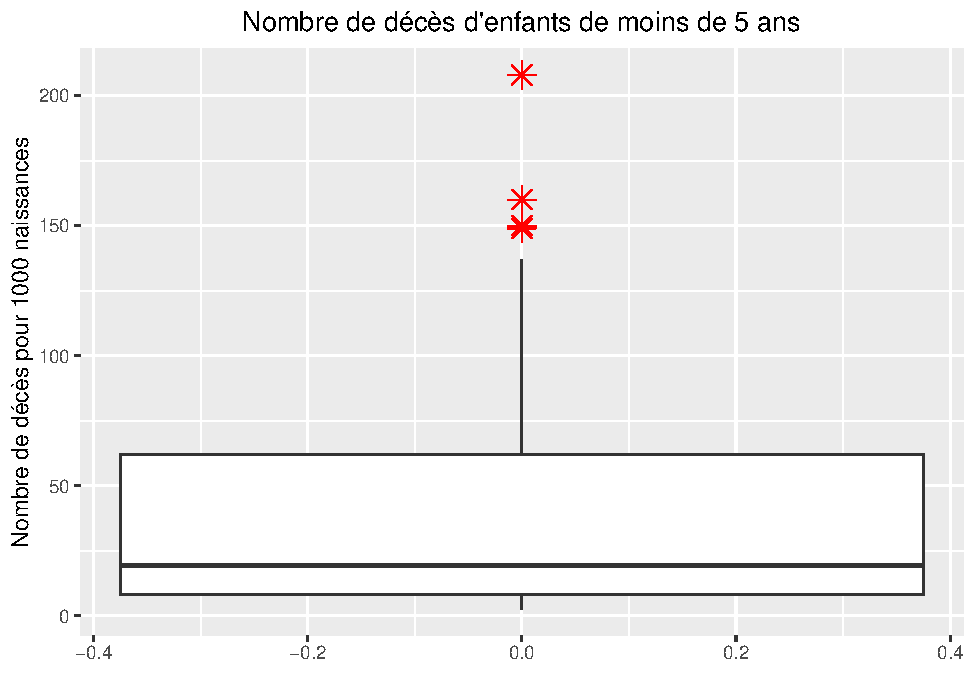
\includegraphics{projet_apprentissage_non_supp_files/figure-latex/unnamed-chunk-5-1.pdf}

\begin{Shaded}
\begin{Highlighting}[]
\NormalTok{sante }\OtherTok{\textless{}{-}} \FunctionTok{ggplot}\NormalTok{(}\AttributeTok{data=}\NormalTok{data, }\FunctionTok{aes}\NormalTok{(}\AttributeTok{y=}\NormalTok{sante)) }\SpecialCharTok{+} 
  \FunctionTok{geom\_boxplot}\NormalTok{(}\AttributeTok{outlier.colour=}\StringTok{"red"}\NormalTok{, }\AttributeTok{outlier.shape=}\DecValTok{8}\NormalTok{,}\AttributeTok{outlier.size=}\DecValTok{4}\NormalTok{)}\SpecialCharTok{+}
  \FunctionTok{labs}\NormalTok{(}\AttributeTok{title=}\StringTok{"Dépenses totales de santé par habitant"}\NormalTok{,}\AttributeTok{y=}\StringTok{"Pourcentage du PIB par habitant"}\NormalTok{)}\SpecialCharTok{+}
  \FunctionTok{theme}\NormalTok{(}\AttributeTok{plot.title =} \FunctionTok{element\_text}\NormalTok{(}\AttributeTok{hjust=}\FloatTok{0.5}\NormalTok{))}

\NormalTok{esperance }\OtherTok{\textless{}{-}} \FunctionTok{ggplot}\NormalTok{(}\AttributeTok{data=}\NormalTok{data, }\FunctionTok{aes}\NormalTok{(}\AttributeTok{y=}\NormalTok{esper\_vie)) }\SpecialCharTok{+} 
  \FunctionTok{geom\_boxplot}\NormalTok{(}\AttributeTok{outlier.colour=}\StringTok{"red"}\NormalTok{, }\AttributeTok{outlier.shape=}\DecValTok{8}\NormalTok{,}\AttributeTok{outlier.size=}\DecValTok{4}\NormalTok{)}\SpecialCharTok{+}
  \FunctionTok{labs}\NormalTok{(}\AttributeTok{title=}\StringTok{"Espérance de vie"}\NormalTok{,}\AttributeTok{y=}\StringTok{"Age"}\NormalTok{)}\SpecialCharTok{+}
  \FunctionTok{theme}\NormalTok{(}\AttributeTok{plot.title =} \FunctionTok{element\_text}\NormalTok{(}\AttributeTok{hjust=}\FloatTok{0.5}\NormalTok{))}

\FunctionTok{grid.arrange}\NormalTok{(sante,esperance,}\AttributeTok{ncol=}\DecValTok{2}\NormalTok{)}
\end{Highlighting}
\end{Shaded}

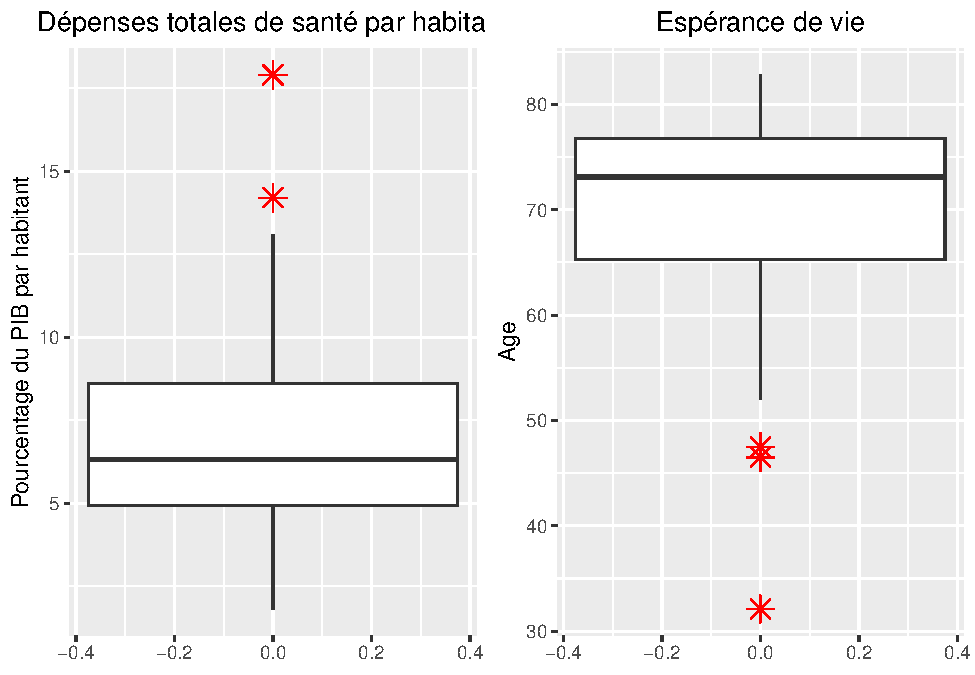
\includegraphics{projet_apprentissage_non_supp_files/figure-latex/unnamed-chunk-6-1.pdf}

\begin{Shaded}
\begin{Highlighting}[]
\NormalTok{revenu\_net }\OtherTok{\textless{}{-}} \FunctionTok{ggplot}\NormalTok{(}\AttributeTok{data=}\NormalTok{data, }\FunctionTok{aes}\NormalTok{(}\AttributeTok{y=}\NormalTok{revenu)) }\SpecialCharTok{+} 
  \FunctionTok{geom\_boxplot}\NormalTok{(}\AttributeTok{outlier.colour=}\StringTok{"red"}\NormalTok{, }\AttributeTok{outlier.shape=}\DecValTok{8}\NormalTok{,}\AttributeTok{outlier.size=}\DecValTok{4}\NormalTok{)}\SpecialCharTok{+}
  \FunctionTok{labs}\NormalTok{(}\AttributeTok{title=}\StringTok{"Revenu net moyen par personne"}\NormalTok{)}\SpecialCharTok{+}
  \FunctionTok{theme}\NormalTok{(}\AttributeTok{plot.title =} \FunctionTok{element\_text}\NormalTok{(}\AttributeTok{hjust=}\FloatTok{0.5}\NormalTok{))}

\NormalTok{pib\_hab }\OtherTok{\textless{}{-}} \FunctionTok{ggplot}\NormalTok{(}\AttributeTok{data=}\NormalTok{data, }\FunctionTok{aes}\NormalTok{(}\AttributeTok{y=}\NormalTok{pib\_h)) }\SpecialCharTok{+} 
  \FunctionTok{geom\_boxplot}\NormalTok{(}\AttributeTok{outlier.colour=}\StringTok{"red"}\NormalTok{, }\AttributeTok{outlier.shape=}\DecValTok{8}\NormalTok{,}\AttributeTok{outlier.size=}\DecValTok{4}\NormalTok{)}\SpecialCharTok{+}
  \FunctionTok{labs}\NormalTok{(}\AttributeTok{title=}\StringTok{"PIB par habitant"}\NormalTok{)}\SpecialCharTok{+}
  \FunctionTok{theme}\NormalTok{(}\AttributeTok{plot.title =} \FunctionTok{element\_text}\NormalTok{(}\AttributeTok{hjust=}\FloatTok{0.5}\NormalTok{))}

\FunctionTok{grid.arrange}\NormalTok{(revenu\_net,pib\_hab,}\AttributeTok{ncol=}\DecValTok{2}\NormalTok{)}
\end{Highlighting}
\end{Shaded}

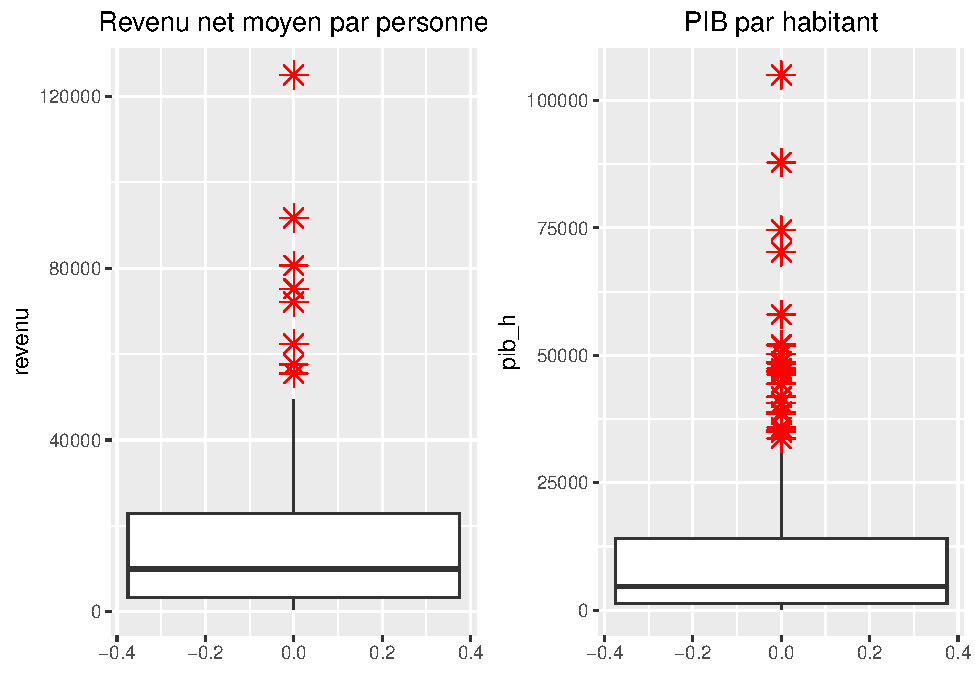
\includegraphics{projet_apprentissage_non_supp_files/figure-latex/unnamed-chunk-7-1.pdf}

\begin{Shaded}
\begin{Highlighting}[]
\FunctionTok{ggplot}\NormalTok{(}\AttributeTok{data=}\NormalTok{data, }\FunctionTok{aes}\NormalTok{(}\AttributeTok{y=}\NormalTok{inflation)) }\SpecialCharTok{+} 
  \FunctionTok{geom\_boxplot}\NormalTok{(}\AttributeTok{outlier.colour=}\StringTok{"red"}\NormalTok{, }\AttributeTok{outlier.shape=}\DecValTok{8}\NormalTok{,}\AttributeTok{outlier.size=}\DecValTok{4}\NormalTok{)}\SpecialCharTok{+}
  \FunctionTok{labs}\NormalTok{(}\AttributeTok{title=}\StringTok{"Mesure du taux de croissance annuel du PIB total"}\NormalTok{)}\SpecialCharTok{+}
  \FunctionTok{theme}\NormalTok{(}\AttributeTok{plot.title =} \FunctionTok{element\_text}\NormalTok{(}\AttributeTok{hjust=}\FloatTok{0.5}\NormalTok{))}
\end{Highlighting}
\end{Shaded}

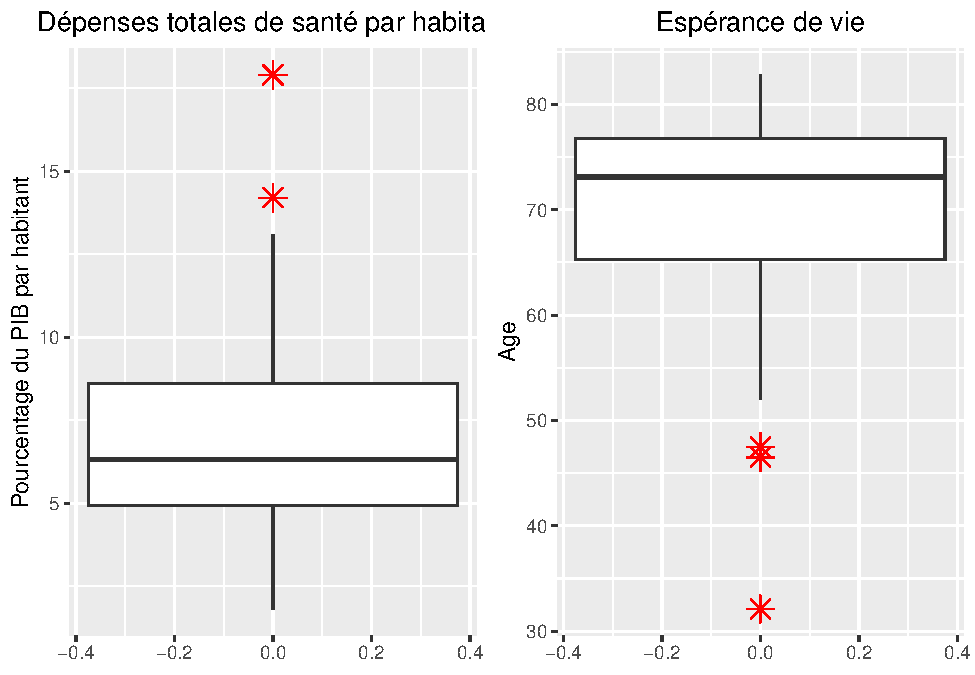
\includegraphics{projet_apprentissage_non_supp_files/figure-latex/unnamed-chunk-8-1.pdf}

\begin{Shaded}
\begin{Highlighting}[]
\FunctionTok{ggplot}\NormalTok{(}\AttributeTok{data=}\NormalTok{data, }\FunctionTok{aes}\NormalTok{(}\AttributeTok{y=}\NormalTok{fert)) }\SpecialCharTok{+} 
  \FunctionTok{geom\_boxplot}\NormalTok{(}\AttributeTok{outlier.colour=}\StringTok{"red"}\NormalTok{, }\AttributeTok{outlier.shape=}\DecValTok{8}\NormalTok{,}\AttributeTok{outlier.size=}\DecValTok{4}\NormalTok{)}\SpecialCharTok{+}
  \FunctionTok{labs}\NormalTok{(}\AttributeTok{title=}\StringTok{"Nombre moyen d\textquotesingle{}enfants par femme"}\NormalTok{)}\SpecialCharTok{+}
  \FunctionTok{theme}\NormalTok{(}\AttributeTok{plot.title =} \FunctionTok{element\_text}\NormalTok{(}\AttributeTok{hjust=}\FloatTok{0.5}\NormalTok{))}
\end{Highlighting}
\end{Shaded}

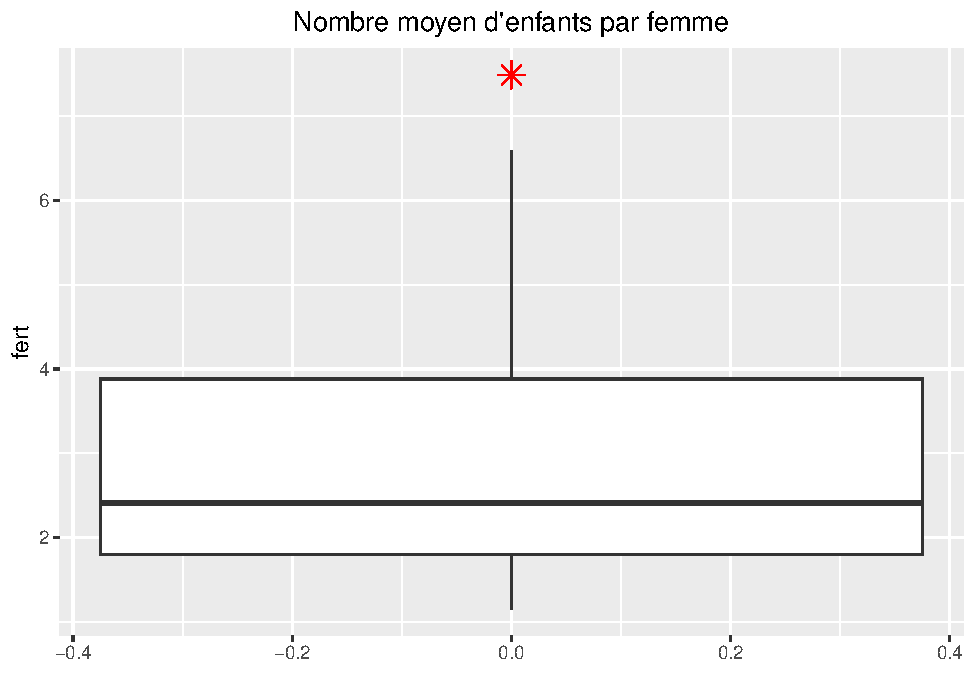
\includegraphics{projet_apprentissage_non_supp_files/figure-latex/unnamed-chunk-9-1.pdf}

Imports et Exports :

\begin{Shaded}
\begin{Highlighting}[]
\NormalTok{imports }\OtherTok{\textless{}{-}} \FunctionTok{ggplot}\NormalTok{(}\AttributeTok{data=}\NormalTok{data, }\FunctionTok{aes}\NormalTok{(}\AttributeTok{y=}\NormalTok{imports)) }\SpecialCharTok{+} 
  \FunctionTok{geom\_boxplot}\NormalTok{(}\AttributeTok{outlier.colour=}\StringTok{"red"}\NormalTok{, }\AttributeTok{outlier.shape=}\DecValTok{8}\NormalTok{,}\AttributeTok{outlier.size=}\DecValTok{4}\NormalTok{)}\SpecialCharTok{+}
  \FunctionTok{labs}\NormalTok{(}\AttributeTok{title=}\StringTok{"Importations de biens et services }\SpecialCharTok{\textbackslash{}n}\StringTok{par habitant"}\NormalTok{,}\AttributeTok{y=}\StringTok{"Pourcentage du PIB par habitant"}\NormalTok{)}\SpecialCharTok{+}
  \FunctionTok{theme}\NormalTok{(}\AttributeTok{plot.title =} \FunctionTok{element\_text}\NormalTok{(}\AttributeTok{hjust=}\FloatTok{0.5}\NormalTok{))}

\NormalTok{exports }\OtherTok{\textless{}{-}} \FunctionTok{ggplot}\NormalTok{(}\AttributeTok{data=}\NormalTok{data, }\FunctionTok{aes}\NormalTok{(}\AttributeTok{y=}\NormalTok{exports)) }\SpecialCharTok{+} 
  \FunctionTok{geom\_boxplot}\NormalTok{(}\AttributeTok{outlier.colour=}\StringTok{"red"}\NormalTok{, }\AttributeTok{outlier.shape=}\DecValTok{8}\NormalTok{,}\AttributeTok{outlier.size=}\DecValTok{4}\NormalTok{)}\SpecialCharTok{+}
  \FunctionTok{labs}\NormalTok{(}\AttributeTok{title=}\StringTok{"Exportations de biens et services }\SpecialCharTok{\textbackslash{}n}\StringTok{par habitant"}\NormalTok{,}\AttributeTok{y=}\StringTok{"Pourcentage du PIB par habitant"}\NormalTok{)}\SpecialCharTok{+}
  \FunctionTok{theme}\NormalTok{(}\AttributeTok{plot.title =} \FunctionTok{element\_text}\NormalTok{(}\AttributeTok{hjust=}\FloatTok{0.5}\NormalTok{))}

\FunctionTok{grid.arrange}\NormalTok{(exports, imports, }\AttributeTok{ncol=}\DecValTok{2}\NormalTok{)}
\end{Highlighting}
\end{Shaded}

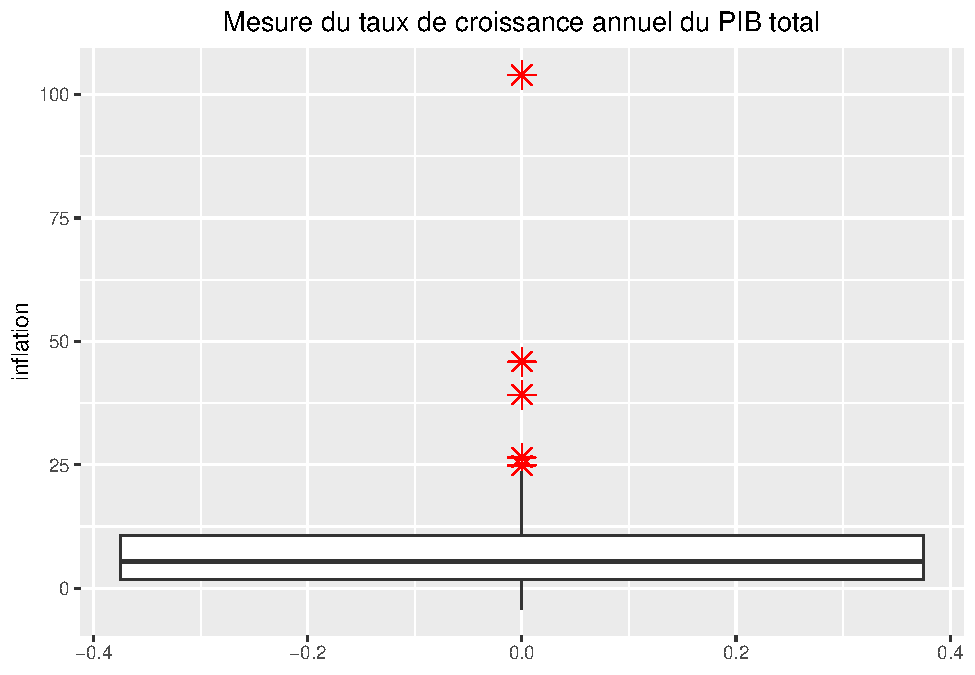
\includegraphics{projet_apprentissage_non_supp_files/figure-latex/unnamed-chunk-10-1.pdf}

\end{document}
